\documentclass[conference,a4paper,twoside]{IEEEtran}
\usepackage[utf8]{inputenc}
\usepackage{amsmath}
\usepackage{amsfonts}
\usepackage{amssymb}
\usepackage{graphicx}
\usepackage[space]{grffile}
\graphicspath{figures/}
\usepackage{import}
\usepackage{url}
\usepackage{hyperref}
\usepackage{subcaption}
\usepackage{tikz}
\usepackage{siunitx}
\usepackage{todonotes}
\let\OldTodo\todo
\renewcommand{\todo}{\OldTodo[inline]}
\newcommand{\todolater}[1]{}%\todo
\RequirePackage[date=terse, isbn=true, doi=true, url=false, urldate=iso8601, maxbibnames=9, backref=false, backend=bibtex]{biblatex}
\addbibresource{securityupdates.bib}
\renewcommand{\bibfont}{\small}

\AtEveryBibitem{% Clean up the bibtex rather than editing it
 \clearname{editor} % remove editors
}

\author{Daniel R.\ Thomas, Alastair R.\ Beresford, Daniel T.\ Wagner and Andrew Rice}

\newcommand{\daNumSigModels}{18}
\newcommand{\daSigNumDevices}{100}
\newcommand{\daSigNumDeviceDays}{10\,000}
\newcommand{\daSigNumDays}{100}
\newcommand{\daSigNumDevicesDay}{20}
\newcommand{\daSigVersionPerc}{1\%}
\newcommand{\daSigVersionDays}{10}
\newcommand{\daNumVulnsUsed}{11}
\newcommand{\daNumDeviceDataDevices}{50}
\newcommand{\daOSYearsOfData}{4}
\newcommand{\daOSMonthsOfData}{51}
\newcommand{\daStartDate}{2011-07-01}
\newcommand{\daEndDate}{2015-09-22}
\newcommand{\daFullDeployedAt}{95\%}
\newcommand{\daNumManufacturers}{302}
\newcommand{\daNumSigManufacturers}{10}
\newcommand{\daNumModels}{2\,770}
\newcommand{\daNumOperators}{1\,470}
\newcommand{\daNumSigOperators}{14}
\newcommand{\daNumOSDevices}{20\,500}
\newcommand{\daOSVersionPercValidLines}{99.9\%}
\newcommand{\daOSTotalDaysData}{1\,350\,000}
\newcommand{\daMeanInsecurityPercNominal}{87.3\%}
\newcommand{\daMeanInsecurityPerc}{$87.3 \pm 0.0\%$}
\newcommand{\daMeanInsecurityPercTwosfNominal}{87\%}
\newcommand{\daMeanInsecurityPercTwosf}{$87 \pm 0\%$}
\newcommand{\daMeanSecurityPercNominal}{12.7\%}
\newcommand{\daMeanSecurityPerc}{$12.7 \pm 0.0\%$}
\newcommand{\daMeanSecurityPercTwosfNominal}{13\%}
\newcommand{\daMeanSecurityPercTwosf}{$13 \pm 0\%$}
\newcommand{\daVulnFreeNominal}{0.127}
\newcommand{\daVulnFree}{$0.127 \pm 0.0$}
\newcommand{\daMeanOutstandingVulnerabilities}{$0.509 \pm 0.0$}
\newcommand{\daUpdatednessNominal}{0.0553}
\newcommand{\daUpdatedness}{$0.0553 \pm 0.0$}
\newcommand{\daUpdatednessPercNominal}{5.53\%}
\newcommand{\daUpdatednessPerc}{$5.53 \pm 0.0\%$}
\newcommand{\daUpdatednessPercTwosfNominal}{5.5\%}
\newcommand{\daUpdatednessPercTwosf}{$5.5 \pm 0.0\%$}
\newcommand{\daSecurityScoreNominal}{2.93}
\newcommand{\daSecurityScore}{$2.93 \pm 0.0$}
\newcommand{\daCurrentMeanInsecurityPercNominal}{68.8\%}
\newcommand{\daCurrentMeanInsecurityPerc}{$68.8 \pm 0.0\%$}
\newcommand{\daCurrentMeanInsecurityPercTwosfNominal}{69\%}
\newcommand{\daCurrentMeanInsecurityPercTwosf}{$69 \pm 0\%$}
\newcommand{\daCurrentMeanSecurityPercNominal}{31.2\%}
\newcommand{\daCurrentMeanSecurityPerc}{$31.2 \pm 0.2\%$}
\newcommand{\daCurrentMeanSecurityPercTwosfNominal}{31\%}
\newcommand{\daCurrentMeanSecurityPercTwosf}{$31 \pm 0\%$}
\newcommand{\daCurrentVulnFreeNominal}{0.312}
\newcommand{\daCurrentVulnFree}{$0.312 \pm 0.002$}
\newcommand{\daCurrentMeanOutstandingVulnerabilities}{$0.0645 \pm 0.0$}
\newcommand{\daCurrentUpdatednessNominal}{0.0934}
\newcommand{\daCurrentUpdatedness}{$0.0934 \pm 0.0019$}
\newcommand{\daCurrentUpdatednessPercNominal}{9.34\%}
\newcommand{\daCurrentUpdatednessPerc}{$9.34 \pm 0.19\%$}
\newcommand{\daCurrentUpdatednessPercTwosfNominal}{9.3\%}
\newcommand{\daCurrentUpdatednessPercTwosf}{$9.3 \pm 0.0\%$}
\newcommand{\daCurrentSecurityScoreNominal}{4.43}
\newcommand{\daCurrentSecurityScore}{$4.43 \pm 0.0$}
\newcommand{\daDailyParticipationNominal}{872}
\newcommand{\daDailyParticipation}{$872 \pm 271$}
\newcommand{\daNumFullVersions}{1\,300}
\newcommand{\daNumSigFullVersions}{101}
\newcommand{\daNumOSVersions}{50}
\newcommand{\daNumSigOSVersions}{28}
\newcommand{\daNumAPIVersions}{16}
\newcommand{\daNumFullVersionUpdates}{4\,670}
\newcommand{\daNumOSVersionUpdates}{3\,940}
\newcommand{\daUpdatesPerYearNominal}{1.27}
\newcommand{\daUpdatesPerYear}{$1.27 \pm 0.01$}
\newcommand{\daUpdatesPerYearTwosfNominal}{1.3}
\newcommand{\daUpdatesPerYearTwosf}{$1.3 \pm 0.0$}
\newcommand{\daNumFullOnlyVersionUpdates}{724}
\newcommand{\daNumSecurityUpdates}{1\,270}
\newcommand{\daNumPossibleSecurityUpdates}{2\,310}
\newcommand{\daOSCurveFitParamFirst}{83.6}
\newcommand{\daOSCurveFitParamSecond}{\num{0.0028}}
\newcommand{\daOSCurveFitRMSE}{0.114}
\newcommand{\daOSCurvePolyRMSE}{0.114}
\newcommand{\daOSCurveSplineRMSE}{0.114}
\newcommand{\daOSCurveHalfDeployedYearsNominal}{0.908}
\newcommand{\daOSCurveHalfDeployedYears}{$0.908 \pm 0.254$}
\newcommand{\daOSCurveHalfDeployedNominal}{332}
\newcommand{\daOSCurveHalfDeployed}{$332 \pm 92$}
\newcommand{\daOSCurveFullDeployedYearsNominal}{3.16}
\newcommand{\daOSCurveFullDeployedYears}{$3.16 \pm 72$}
\newcommand{\daOSCurveFullDeployedNominal}{1\,150}
\newcommand{\daOSCurveFullDeployed}{$1\,150 \pm 265\,000$}
\newcommand{\daAPICurveFitParamFirst}{97.8}
\newcommand{\daAPICurveFitParamSecond}{\num{0.0028}}
\newcommand{\daAPICurveFitRMSE}{0.11}
\newcommand{\daAPICurvePolyRMSE}{0.111}
\newcommand{\daAPICurveSplineRMSE}{0.111}
\newcommand{\daAPICurveHalfDeployedYearsNominal}{0.946}
\newcommand{\daAPICurveHalfDeployedYears}{$0.946 \pm 0.244$}
\newcommand{\daAPICurveHalfDeployedNominal}{345}
\newcommand{\daAPICurveHalfDeployed}{$345 \pm 89$}
\newcommand{\daAPICurveFullDeployedYearsNominal}{3.2}
\newcommand{\daAPICurveFullDeployedYears}{$3.2 \pm 7$}
\newcommand{\daAPICurveFullDeployedNominal}{1\,170}
\newcommand{\daAPICurveFullDeployed}{$1\,170 \pm 265\,000$}
\newcommand{\daVulnAPKDuplicateFileOctoberPerc}{91.7\%}
\newcommand{\daVulnZergRushMonthsDefFixDeployed}{27.3}
\newcommand{\daTabSecScoresmanufacturer}{\begin{table*} \centering \begin{tabular}{l|c|c|c|c} Name & $f$ & $u$ & $m$ & \textbf{score} \\ &&&& (out of 10) \\ \hline LG & $0.24 \pm 0.00$ & $0.34 \pm 0.00$ & $0.60 \pm 0.01$ & $4.11 \pm 0.02$ \\  Motorola & $0.19 \pm 0.00$ & $0.12 \pm 0.00$ & $0.71 \pm 0.02$ & $3.11 \pm 0.02$ \\  Samsung & $0.13 \pm 0.00$ & $0.04 \pm 0.00$ & $0.58 \pm 0.00$ & $2.80 \pm 0.00$ \\  Sony & $0.14 \pm 0.00$ & $0.19 \pm 0.00$ & $1.09 \pm 0.02$ & $2.66 \pm 0.02$ \\  HTC & $0.14 \pm 0.00$ & $0.10 \pm 0.00$ & $0.86 \pm 0.01$ & $2.65 \pm 0.02$ \\  asus & $0.21 \pm 0.00$ & $0.51 \pm 0.01$ & $6.01 \pm 0.07$ & $2.38 \pm 0.02$ \\  other & $0.06 \pm 0.00$ & $0.05 \pm 0.00$ & $1.00 \pm 0.01$ & $2.02 \pm 0.02$ \\  alps & $0.03 \pm 0.00$ & $0.19 \pm 0.01$ & $3.99 \pm 0.08$ & $0.80 \pm 0.02$ \\  Symphony & $0.00 \pm 0.00$ & $0.09 \pm 0.00$ & $5.00 \pm 0.05$ & $0.32 \pm 0.01$ \\  walton & $0.00 \pm 0.00$ & $0.09 \pm 0.00$ & $6.00 \pm 0.08$ & $0.27 \pm 0.01$ \\ \end{tabular} \caption{Security scores for manufacturers} \label{tab:sec_manufacturer} \end{table*}}
\newcommand{\daSecScoreBestmanufacturer}{LG}
\newcommand{\daSecScoreBestmanufacturerScoreNominal}{4.11}
\newcommand{\daSecScoreBestmanufacturerScore}{$4.11 \pm 0.0$}
\newcommand{\daSecScoreBestmanufacturerNumFullVersions}{142}
\newcommand{\daSecScoreWorstmanufacturer}{walton}
\newcommand{\daSecScoreWorstmanufacturerScoreNominal}{0.273}
\newcommand{\daSecScoreWorstmanufacturerScore}{$0.273 \pm 0.007$}
\newcommand{\daSecScoreWorstmanufacturerNumFullVersions}{21}
\newcommand{\daTabSecScoresmodel}{\begin{table*} \centering \begin{tabular}{l|c|c|c|c} Name & $f$ & $u$ & $m$ & \textbf{score} \\ &&&& (out of 10) \\ \hline Galaxy Nexus & $0.50 \pm 0.00$ & $0.54 \pm 0.01$ & $1.53 \pm 0.04$ & $4.70 \pm 0.04$ \\  Nexus 4 & $0.33 \pm 0.00$ & $0.82 \pm 0.01$ & $6.06 \pm 0.09$ & $3.78 \pm 0.04$ \\  Nexus 7 & $0.27 \pm 0.00$ & $0.73 \pm 0.01$ & $5.92 \pm 0.09$ & $3.29 \pm 0.04$ \\  other & $0.10 \pm 0.00$ & $0.14 \pm 0.00$ & $0.51 \pm 0.00$ & $3.08 \pm 0.00$ \\  Desire HD & $0.08 \pm 0.00$ & $0.05 \pm 0.00$ & $0.38 \pm 0.02$ & $2.91 \pm 0.04$ \\  HTC Sensation & $0.35 \pm 0.00$ & $0.01 \pm 0.01$ & $1.57 \pm 0.05$ & $2.44 \pm 0.05$ \\  GT-I9100 & $0.22 \pm 0.00$ & $0.02 \pm 0.00$ & $1.23 \pm 0.02$ & $2.27 \pm 0.02$ \\  HTC Desire S & $0.02 \pm 0.00$ & $0.02 \pm 0.00$ & $1.00 \pm 0.06$ & $1.74 \pm 0.07$ \\  GT-N7000 & $0.25 \pm 0.00$ & $0.00 \pm 0.00$ & $2.52 \pm 0.05$ & $1.43 \pm 0.02$ \\  GT-P1000 & $0.01 \pm 0.00$ & $0.00 \pm 0.01$ & $1.79 \pm 0.06$ & $0.90 \pm 0.05$ \\  GT-I9505 & $0.06 \pm 0.00$ & $0.13 \pm 0.00$ & $6.82 \pm 0.07$ & $0.62 \pm 0.01$ \\  GT-I9300 & $0.13 \pm 0.00$ & $0.01 \pm 0.00$ & $6.23 \pm 0.04$ & $0.57 \pm 0.01$ \\  HTC Desire HD & $0.00 \pm 0.00$ & $0.00 \pm 0.01$ & $3.03 \pm 0.05$ & $0.28 \pm 0.03$ \\  GT-N7100 & $0.06 \pm 0.00$ & $0.00 \pm 0.01$ & $6.93 \pm 0.08$ & $0.24 \pm 0.02$ \\  Symphony W68 & $0.00 \pm 0.00$ & $0.00 \pm 0.01$ & $11.00 \pm 0.12$ & $0.00 \pm 0.03$ \\ \end{tabular} \caption{Security scores for models} \label{tab:sec_model} \end{table*}}
\newcommand{\daSecScoreBestmodel}{Galaxy Nexus}
\newcommand{\daSecScoreBestmodelScoreNominal}{4.7}
\newcommand{\daSecScoreBestmodelScore}{$4.7 \pm 0.0$}
\newcommand{\daSecScoreBestmodelNumFullVersions}{49}
\newcommand{\daSecScoreWorstmodel}{Symphony W68}
\newcommand{\daSecScoreWorstmodelScoreNominal}{0.0001}
\newcommand{\daSecScoreWorstmodelScore}{$0.0001 \pm 0.0272$}
\newcommand{\daSecScoreWorstmodelNumFullVersions}{1}
\newcommand{\daTabSecScoressummary}{\begin{table*} \centering \begin{tabular}{l|c|c|c|c} Name & $f$ & $u$ & $m$ & \textbf{score} \\ &&&& (out of 10) \\ \hline nexus & $0.40 \pm 0.00$ & $0.49 \pm 0.00$ & $0.55 \pm 0.01$ & $5.28 \pm 0.02$ \\  non-nexus & $0.11 \pm 0.00$ & $0.03 \pm 0.00$ & $0.51 \pm 0.00$ & $2.76 \pm 0.00$ \\ \end{tabular} \caption{Security scores for nexus} \label{tab:sec_summary} \end{table*}}
\newcommand{\daTabSecScoresoperator}{\begin{table*} \centering \begin{tabular}{l|c|c|c|c} Name & $f$ & $u$ & $m$ & \textbf{score} \\ &&&& (out of 10) \\ \hline O2 uk & $0.28 \pm 0.00$ & $0.12 \pm 0.00$ & $0.37 \pm 0.02$ & $3.91 \pm 0.03$ \\  T-Mobile & $0.22 \pm 0.00$ & $0.19 \pm 0.00$ & $0.39 \pm 0.01$ & $3.87 \pm 0.02$ \\  Orange & $0.22 \pm 0.00$ & $0.10 \pm 0.00$ & $0.36 \pm 0.02$ & $3.64 \pm 0.04$ \\  3 & $0.22 \pm 0.00$ & $0.09 \pm 0.00$ & $0.47 \pm 0.02$ & $3.45 \pm 0.03$ \\  Sprint & $0.18 \pm 0.00$ & $0.11 \pm 0.00$ & $0.43 \pm 0.02$ & $3.41 \pm 0.03$ \\  Vodafone uk & $0.14 \pm 0.00$ & $0.13 \pm 0.00$ & $0.52 \pm 0.03$ & $3.19 \pm 0.04$ \\  AT\&T & $0.15 \pm 0.00$ & $0.08 \pm 0.00$ & $0.43 \pm 0.02$ & $3.17 \pm 0.02$ \\  unknown & $0.12 \pm 0.00$ & $0.20 \pm 0.00$ & $0.80 \pm 0.01$ & $2.95 \pm 0.02$ \\  Verizon & $0.19 \pm 0.00$ & $0.09 \pm 0.00$ & $0.82 \pm 0.02$ & $2.86 \pm 0.02$ \\  n Telenor & $0.05 \pm 0.00$ & $0.12 \pm 0.00$ & $1.14 \pm 0.02$ & $2.01 \pm 0.02$ \\  Airtel & $0.05 \pm 0.00$ & $0.03 \pm 0.00$ & $1.44 \pm 0.03$ & $1.45 \pm 0.03$ \\  Grameenphone & $0.01 \pm 0.00$ & $0.04 \pm 0.00$ & $1.66 \pm 0.02$ & $1.10 \pm 0.01$ \\  Robi & $0.00 \pm 0.00$ & $0.08 \pm 0.00$ & $2.08 \pm 0.04$ & $0.91 \pm 0.03$ \\  banglalink & $0.00 \pm 0.00$ & $0.04 \pm 0.00$ & $2.55 \pm 0.04$ & $0.55 \pm 0.02$ \\ \end{tabular} \caption{Security scores for operators} \label{tab:sec_operator} \end{table*}}
\newcommand{\daSecScoreBestoperator}{O2 uk}
\newcommand{\daSecScoreBestoperatorScoreNominal}{3.91}
\newcommand{\daSecScoreBestoperatorScore}{$3.91 \pm 0.0$}
\newcommand{\daSecScoreBestoperatorNumFullVersions}{103}
\newcommand{\daSecScoreWorstoperator}{banglalink}
\newcommand{\daSecScoreWorstoperatorScoreNominal}{0.547}
\newcommand{\daSecScoreWorstoperatorScore}{$0.547 \pm 0.017$}
\newcommand{\daSecScoreWorstoperatorNumFullVersions}{75}
\newcommand{\daTabDLDistances}{\begin{table} \centering \begin{tabular}{l|c|c|c|c} & manufacturer & model & operator & nexus \\ \hline equal & 0.0 & 0.0 & 0.0714 & 0.0 \\weight $m$ & 0.2 & 0.333 & 0.214 & 0.0 \\weight $u$ & 0.2 & 0.0 & 0.143 & 0.0 \\$f$ & 0.3 & 0.733 & 0.357 & 0.0 \\$m$ & 0.6 & 0.733 & 0.357 & 0.5 \\$u$ & 0.9 & 0.667 & 0.786 & 0.0 \\\end{tabular} \caption{Normalised Damerau-Levenshtein distances for different metrics} \label{tab:dl_distances} \end{table}}
\newcommand{\daTabChangeInScores}{\begin{table*}\small \centering \begin{tabular}{l|c|c|c|c} & manufacturer & model & operator & nexus \\ \hline $m$ & $-1.67 \pm 2.26$ & $-0.65 \pm 2.56$ & $-3.34 \pm 1.27$ & $-3.4 \pm 1.9$ \\weight $m$ & $-0.263 \pm 0.278$ & $-0.0958 \pm 0.325$ & $-0.464 \pm 0.159$ & $-0.488 \pm 0.225$ \\equal & $-0.106 \pm 0.061$ & $-0.0343 \pm 0.111$ & $-0.145 \pm 0.043$ & $-0.164 \pm 0.035$ \\weight $u$ & $-0.0569 \pm 0.121$ & $-0.00706 \pm 0.225$ & $0.029 \pm 0.082$ & $-0.00391 \pm 0.12$ \\$u$ & $0.389 \pm 1.62$ & $0.238 \pm 2.09$ & $1.6 \pm 0.9$ & $1.44 \pm 1.51$ \\$f$ & $0.958 \pm 0.556$ & $0.309 \pm 1.0$ & $1.31 \pm 0.39$ & $1.48 \pm 0.32$ \\\end{tabular} \caption{Mean change in scores for different metrics} \label{tab:change_in_scores} \end{table*}}
\newcommand{\daGPAPICurveFitParamFirst}{82.1}
\newcommand{\daGPAPICurveFitParamSecond}{\num{0.00257}}
\newcommand{\daGPAPICurveFitRMSE}{0.176}
\newcommand{\daGPAPICurvePolyRMSE}{0.176}
\newcommand{\daGPAPICurveSplineRMSE}{0.176}
\newcommand{\daGPAPICurveHalfDeployedYearsNominal}{0.964}
\newcommand{\daGPAPICurveHalfDeployedYears}{$0.964 \pm 0.462$}
\newcommand{\daGPAPICurveHalfDeployedNominal}{352}
\newcommand{\daGPAPICurveHalfDeployed}{$352 \pm 169$}
\newcommand{\daGPAPICurveFullDeployedYearsNominal}{3.42}
\newcommand{\daGPAPICurveFullDeployedYears}{$3.42 \pm 79$}
\newcommand{\daGPAPICurveFullDeployedNominal}{1\,250}
\newcommand{\daGPAPICurveFullDeployed}{$1\,250 \pm 289\,000$}
\newcommand{\daGPAPIPerAPIMeanNominal}{0.00472}
\newcommand{\daGPAPIPerAPIMean}{$0.00472 \pm 0.00327$}
\newcommand{\daGPAPIPerAPIStdevNominal}{0.0209}
\newcommand{\daGPAPIPerAPIStdev}{$0.0209 \pm 0.0121$}
\newcommand{\daGPAPIPerAPIAbsMeanNominal}{0.0143}
\newcommand{\daGPAPIPerAPIAbsMean}{$0.0143 \pm 0.0066$}
\newcommand{\daGPAPIPerAPIAbsStdevNominal}{0.0155}
\newcommand{\daGPAPIPerAPIAbsStdev}{$0.0155 \pm 0.0112$}
\newcommand{\daGPAPIPerAPIParametersTable}{\begin{table} \centering \begin{tabular}{c|S|S} API Version & ${t_0}$ & $\mathrm{decay}$ \\ \hline2	&	0.0	&	0.0237\\3	&	0.0	&	0.0235\\4	&	0.0	&	0.00689\\5	&	36.3	&	0.00429\\6	&	0.0	&	0.0043\\7	&	0.0	&	0.00499\\8	&	47.7	&	0.00415\\9	&	155	&	0.00365\\10	&	90.3	&	0.00364\\11	&	445	&	0.00236\\12	&	356	&	0.00229\\13	&	305	&	0.00237\\14	&	219	&	0.0024\\15	&	161	&	0.00241\\16	&	143	&	0.00229\\17	&	292	&	0.00199\\18	&	136	&	0.00152\\19	&	123	&	0.00158\\\end{tabular} \caption{Parameters for different API versions} \label{tab:per_api_parameters} \end{table}}
\newcommand{\daGPAPISeventeenLaterDate}{2015-09-07}
\newcommand{\daGPAPISeventeenLaterProportion}{79.9\%}
\newcommand{\daGPAPISeventeenEarlierProportion}{20.1\%}
\newcommand{\daAPISeventeenReleaseDate}{2012-10-29}
\newcommand{\daGPAPISeventeenFullDeployment}{2017-09-28}
\newcommand{\daGPAPISeventeenCurveFitParamFirst}{292}
\newcommand{\daGPAPISeventeenCurveFitParamSecond}{\num{0.00199}}
\newcommand{\daGPAPISeventeenCurveFitRMSE}{0.027}
\newcommand{\daGPAPISeventeenCurvePolyRMSE}{0.0103}
\newcommand{\daGPAPISeventeenCurveSplineRMSE}{0.0103}
\newcommand{\daGPAPISeventeenCurveHalfDeployedYearsNominal}{1.75}
\newcommand{\daGPAPISeventeenCurveHalfDeployedYears}{$1.75 \pm 0.07$}
\newcommand{\daGPAPISeventeenCurveHalfDeployedNominal}{639}
\newcommand{\daGPAPISeventeenCurveHalfDeployed}{$639 \pm 27$}
\newcommand{\daGPAPISeventeenCurveFullDeployedYearsNominal}{4.92}
\newcommand{\daGPAPISeventeenCurveFullDeployedYears}{$4.92 \pm 1.07$}
\newcommand{\daGPAPISeventeenCurveFullDeployedNominal}{1\,800}
\newcommand{\daGPAPISeventeenCurveFullDeployed}{$1\,800 \pm 390$}
\newcommand{\daNumUpdatesUpgrades}{3\,690}
\newcommand{\daUpdatesPerMonthPerVersionNominal}{2.59}
\newcommand{\daUpdatesPerMonthPerVersion}{$2.59 \pm 0.04$}
\newcommand{\daNumUpdatesSkippedBig}{3}
\newcommand{\daNumUpdatesBigUpgrades}{843}
\newcommand{\daNumUpdatesDowngrades}{146}
\newcommand{\daNumUpdateFullOnly}{721}
\newcommand{\daPercBigUpgradesNominal}{18.5\%}
\newcommand{\daPercBigUpgrades}{$18.5 \pm 0.6\%$}
\newcommand{\daPercUpdatesDowngradesNominal}{3.2\%}
\newcommand{\daPercUpdatesDowngrades}{$3.2 \pm 0.2\%$}
\newcommand{\daNumDataPoints}{103 billion}
\newcommand{\daMonthsDevices}{2\,140}
\newcommand{\daMonths}{6}
\newcommand{\daAdbEnabledPercNominal}{19.2\%}
\newcommand{\daAdbEnabledPerc}{$19.2 \pm 0.0\%$}
\newcommand{\daNumStartedApps}{129\,000}
\newcommand{\daNumInstalledApps}{184\,000}
\newcommand{\daAPISeventeenReleaseDateMonth}{October 2012}
\newcommand{\daGPAPISeventeenFullDeploymentMonth}{September 2017}
\newcommand{\daMeanOutstandingVulnerabilitiesNominal}{0.509}
\newcommand{\daCurrentMeanOutstandingVulnerabilitiesNominal}{0.0645}
\newcommand{\daModelHalfDeploymentYears}{0.0822}
\newcommand{\daModelHalfDeployment}{30}
\newcommand{\daModelFullDeploymentYears}{0.888}
\newcommand{\daModelFullDeployment}{324}
\newcommand{\daMeanOutstandingProbability}{1.0\%}
\newcommand{\daMeanOutstandingUncertaintyEquation}{$0.99^n$}
\newcommand{\daGPAPISeventeenLaterDateMonth}{September 2015}
\newcommand{\daTabSpearmanRanks}{\begin{table} \centering \begin{tabular}{l|c|c|c|c} & manufacturer & model & operator & nexus \\ $\pm\sigma$ & 0.211 & 0.169 & 0.175 & 0.632 \\ \hline $u$ & 0.309 & 0.8 & 0.609 & 1.0 \\$m$ & 0.794 & 0.589 & 0.965 & -1.0 \\$f$ & 0.842 & 0.754 & 0.943 & 1.0 \\weight $m$ & 0.976 & 0.968 & 0.987 & 1.0 \\weight $u$ & 0.976 & 1.0 & 0.991 & 1.0 \\equal & 1.0 & 1.0 & 0.996 & 1.0 \\\end{tabular} \caption{Spearman Rank correlation coefficients for different metrics. The uncertainty is constant for each column but does not take into account the uncertainty in the score which produced the ranking.} \label{tab:spearman_ranks} \end{table}}
\newcommand{\daStartDateMonth}{July 2011}
\newcommand{\daEndDateMonth}{September 2015}
\newcommand{\daSecScoreBestsummary}{nexus}
\newcommand{\daSecScoreBestsummaryScoreNominal}{5.28}
\newcommand{\daSecScoreBestsummaryScore}{$5.28 \pm 0.0$}
\newcommand{\daSecScoreBestsummaryNumFullVersions}{99}
\newcommand{\daSecScoreWorstsummary}{non-nexus}
\newcommand{\daSecScoreWorstsummaryScoreNominal}{2.76}
\newcommand{\daSecScoreWorstsummaryScore}{$2.76 \pm 0.0$}
\newcommand{\daSecScoreWorstsummaryNumFullVersions}{1\,280}

\newcommand{\da}{Device Analyzer}
\newcommand{\dafoot}{\textsuperscript{\ref{foot:dadata}}}
\newcommand{\avoNumSubmitters}{7}
\newcommand{\avoTotalExternalLines}{25 Million}
\newcommand{\avoNumExternalProjects}{176}
\newcommand{\avoNumBigExternalLinesOfCode}{25 Million}
\newcommand{\avoBigExternalLinesOfCodePerc}{99.7\%}
\newcommand{\avoNumVulnerabilities}{31}
\newcommand{\avoNumVulnAllAndroid}{15}
\newcommand{\avoNumVulnSpecific}{16}
\newcommand{\avoStartDate}{2013-08-28}
\newcommand{\avoEndDate}{2014-10-17}
\newcommand{\avoFirstDataDate}{2010-07-13}
\newcommand{\avoLastDataDate}{2014-07-29}
\newcommand{\avoVulnsPerYearNominal}{7.66}
\newcommand{\avoVulnsPerYear}{$7.66 \pm 1.38$}
\newcommand{\avoVulnsPerYearAllAndroidNominal}{3.71}
\newcommand{\avoVulnsPerYearAllAndroid}{$3.71 \pm 0.95$}
\newcommand{\avoTabAndVulns}{\begin{table} \centering \small \begin{tabular}{l|l|c|c} Vulnerability & How known & Date & Categories\\ \hline KillingInTheNameOf & Fixed on & 2010-07-13 & system, kernel\\ exploid udev & Discovered on & 2010-07-15 & kernel\\ levitator & Discovered on & 2011-03-10 & kernel\\ Gingerbreak & Fixed on & 2011-04-18 & system\\ zergRush & Discovered on & 2011-10-06 & system\\ APK duplicate file & Discovered on & 2013-02-18 & signature\\ APK unchecked name & Discovered on & 2013-06-30 & signature\\ APK unsigned shorts & Fixed on & 2013-07-03 & signature\\ vold asec & Fixed on & 2014-01-27 & system\\ Fake ID & Fixed on & 2014-04-17 & signature\\ TowelRoot & Discovered on & 2014-05-03 & kernel\\\end{tabular} \caption{Critical vulnerabilities in Android} \label{tab:andvulns} \end{table}}
\newcommand{\avoNumBigExternalProjects}{40}
\newcommand{\avoNumAnalysedExternalProjects}{28}
\newcommand{\avoNumAnalysedExternalLinesOfCode}{6 Million}
\newcommand{\avoAnalysedExternalLinesOfCodePerc}{24.9\%}
\newcommand{\avoBigExternalMedianVersions}{1.5}
\newcommand{\avoBigExternalMeanVersionsNominal}{2.07}
\newcommand{\avoBigExternalMeanVersions}{$2.07 \pm 1.44$}
\newcommand{\avoBigExternalTotalVersions}{58}

\newcommand{\avo}{\texttt{androidvulnerabilities.org}}
\newcommand{\percMarketShare}{XX\%~\cite{TODO}}
\newcommand{\daNumDevices}{\daNumOSDevices}
\newcommand{\daDeviceDays}{\daOSTotalDaysData}
% Num versions since \daStartDate
\newcommand{\opensslNumVersions}{51}
\newcommand{\linuxNumVersions}{478}
\newcommand{\linuxMeanUpdateLatency}{$137 \pm 48.9$}
\newcommand{\opensslMeanUpdateLatency}{$108 \pm 63.6$}
\newcommand{\bouncycastleNumVersions}{5}
\newcommand{\bouncycastleMeanUpdateLatency}{$220 \pm 70.4$}
\newcommand{\linuxMeanUpdateLatencyNominal}{137}
\newcommand{\opensslMeanUpdateLatencyNominal}{108}
\newcommand{\bouncycastleMeanUpdateLatencyNominal}{220}

\newcommand{\otherProjNumVersions}{XXX}
\newcommand{\otherProjNum}{\avoNumExternalProjects}%TODO check we are doing the right calculation here and not overcounting

\begin{document}
\title{Timeliness of security updates for Android}


% author names and affiliations
% use a multiple column layout for up to three different
% affiliations
\author{
\IEEEauthorblockN{Daniel R. Thomas,
Daniel T. Wagner,
Alastair R. Beresford,
Andrew Rice}
\IEEEauthorblockA{
Computer Laboratory\\
University of Cambridge\\
Cambridge, United Kingdom\\
Firstname.Lastname@cl.cam.ac.uk
}
}

% Terminology

% Android, Unix


\maketitle

% Hypothesis
% Attempts at fine grained restrictions on running arbitrary code are hampered by updates for security vulnerabilities not reaching users in a timely fashion.

\begin{abstract}
Android is the most popular smartphone platform and seeks to provide better security than popular desktop operating systems through increased compartmentalisation and a permission system for apps.
This security relies on the absence of root privilege exploits which allow apps to bypass protections.
Many such exploits have been found and fixed.
Our hypothesis is that these fixes do not promptly reach the users devices and so much of the time users are running versions of Android known to be vulnerable.
We used \da\ data from over \daOSYearsOfData\ years and \daNumOSDevices\ devices and found that on average over \daMeanInsecurityPerc\ of devices were exposed to known root privilege vulnerabilities and only \daUpdatednessPerc\ of devices run the most recent version of Android.
There was also a period of several months when no devices ran secure versions of Android.
We compare different manufacturers and operators to find which are best at promptly distributing security updates and examine how to improve the situation. %TODO operators analysis
\end{abstract}

\section{Introduction}
Android has \percMarketShare\ of the smartphone market and while the core development is controlled by Google there are about \daNumManufacturers\footnote{\label{foot:dadata}We computed this from the \da~\cite{Wagner2013} data, see \S\ref{sec:android_update_process}.} manufacturers which make devices which run Android.
Android receives regular updates  which add new features and fix bugs, including security vulnerabilities.
Many of these manufacturers customise the version of Android they ship and sometimes network operators (of which there are at least \daNumOperators\dafoot) make further modifications.
Hence when Google produces an update to Android, the update may have to pass through the manufacturer and operator before reaching the user.
The manufacturer and operator have little financial incentive to perform this work as they have already sold the device.
Operators are cautious because if they ship a broken update then they will get many support requests which is expensive.
However there is ongoing legal action to force operators to ship updates for security vulnerabilities~\cite{Soghoian2013}.\todolater{Check on the status of this legal action}
Many phones are sold on long (12--24 month) contracts with monthly payments yet stop receiving updates before the end of the contract,\todolater{Is there a survey of the distribution of contract lengths and phone purchase methods?} while Windows XP could be purchased for a one off payment in October 2001 and received security updates until April 2014.
Corporate or public sector buyers are encouraged to purchase secure devices, but we have found little concrete guidance. For example, CESG, which advises the UK government on how to secure its computer systems, recommends picking Android devices from manufactures which are good at shipping security updates promptly~\cite{CESG2013} but it does not state which manufacturers are better.\todolater{Which other advisory organisations give that advice?}
We provide this information in~\S\ref{sec:security_scoring}.

Android relies on the Linux kernel to provide compartmentalisation and runs each app as a separate Unix `user'.
The Linux kernel is a large piece of software and so there will always be new root exploits found in it~\cite{TODO}.
Manufacturers of Android devices have also added further root exploits when customising it~\cite{Grace2012}.
Between 36.7\%~\cite{Zhou2012b} and 40\%~\cite{Zhou2012a} of malware for Android contained root exploits in 2012.
While this shows that much Android malware does not need a root exploit to work, since the user will grant the relevant permissions if the app requests them, a significant proportion does use root exploits.
This malware is also more dangerous because while ordinary malware can be remotely removed by Google through the Play store, once a root exploit has been used there are no guarantees.

The proportion of Android devices in the \da\ data which were running versions of Android known to have root vulnerabilities at the time is shown in Figure~\ref{fig:proportioninsecure}.

\begin{figure}[!b]
\centering
\includegraphics[width=\columnwidth]{figures/proportioninsecure}
%TODO make this graph shorter
\caption{Proportion of devices running insecure versions of Android against time}
\label{fig:proportioninsecure}
\end{figure}

In the past users of Microsoft IIS were advised to switch to a different web server due to the frequent discovery of vulnerabilities~\cite{Pescatore2001}.
This pressure encouraged Microsoft to improve the security of their products~\cite{TODO}.
Part of the reason why deployed devices do not receive updates in a timely manner is that there is little data on what is actually happening and so it is not possible to determine which manufacturers or operators are doing a better job.
Hence there is little incentive for manufacturers and operators to do a better job.
We provide this data  in~\S\ref{sec:security_scoring} and discuss incentives further in \S\ref{sec:economics}.

The contributions of this paper are:
\begin{itemize}
 \item We characterise the Android update ecosystem and quantify its vulnerability to root equivalent vulnerabilities.
 \item We collate information on vulnerabilities which affect Android and investigate their time-lines.
 \item We measure the security of Android according to three metrics and compare different manufacturers. and device models to allow consumers to differentiate between them based on security.
 \item We provide models of how the distribution of Android versions changes allowing future version distributions to be predicted.
% \item We propose methods which could be used to improve the situation in future.
\end{itemize}

\section{Background}
\label{sec:background}
There are two sources of data we needed to have and to link for this study, information on the distribution of installed versions of Android over time and on root vulnerabilities.
We need data on root vulnerabilities so that we know which versions of Android were vulnerable to which known vulnerabilities at what times.
We need information on the distribution of installed versions of Android so that we know what proportion of Android devices were affected by these vulnerabilities.


\subsection{Versions of Android running on devices}
We need historical data on the distributions of versions of Android running on devices and additional data about those devices to allows us to investigate variation between devices and confirm the reliability of these data.
The only suitable data which is available for this is the \da\ data~\cite{Wagner2013}.
The \da\ data contains data from \daNumDevices\ devices with a total of \daDeviceDays\footnote{Here we are only counting devices and days for which we have valid OS version data} device days, it contains data for more than \daMonths\ months for \daMonthsDevices\ devices.
Device Analyzer used an Android app which volunteers install on their Android devices to collect data on what happens on Android phones.
The data collected is available for researchers to use as we do here.

Various different kinds of data\footnote{\url{https://deviceanalyzer.cl.cam.ac.uk/collected.htm}} are collected by the \da\ Android app\footnote{\url{https://deviceanalyzer.cl.cam.ac.uk/}}.
Among these are the build string and API version for the version of Android currently running on the device each day.
The API version is a well defined integer, however it does not always change with new Android releases, particularly security bug fixes should not increase this value.
The build string is `The user-visible version string', fortunately most (99.9\%)\todolater{use a generated number} devices in the data have a build string of the form `x.y.z random string' and so it is possible to extract the Android version number.
On a large proportion of devices `random string' is a well defined build number\footnote{\url{https://source.android.com/source/build-numbers.html}} but different manufacturers use different schema.


\subsection{Root vulnerabilities}
We compiled a list of root equivalent vulnerabilities in Android.
We collected information on discovery and publication dates, what versions they affected and which versions fixed the problem.
We only looked for \emph{root equivalent} vulnerabilities which did not require USB debugging to exploit.
\emph{Root equivalent} means that it escalates to privileges equivalent in scope to root in that either they can be used to gain root or they provide permissions as bad as root.
If an application exploits a root equivalent vulnerability then it gains control of the device.
Some phones can be `rooted' by enabling USB debugging and using the special privileges of the adb shell to root the device but only \daAdbEnabledPerc\dafoot\ of devices have USB debugging enabled.\footnote{This is surprisingly high as \daAdbEnabledPerc\ of Android users are not developers.}
This is not something that applications running on the phone can exploit to break compartmentalisation and so we do not include those vulnerabilities.
Unfortunately many published exploits use adb for convenience and so determining whether that is necessary to exploit the vulnerability can be difficult.

Some vulnerabilities which grant root are not traditional kernel vulnerabilities, for example the discovery of flaws in the verification of signatures on Android applications in February 2013~\cite{Forristal2013} meant that applications could pretend to be signed with system keys and hence gain root equivalent privileges.
On some versions of Android (below 4.1) they could use known system to root escalation mechanisms but on all versions they have a greatly increased attack area for further privilege escalation and also have the ability to control all user internet traffic (via VPNs), brick the phone, remove and install apps, steal user credentials, read the screen and make as well as receive calls.

\avoTabAndVulns

We developed and maintain an open platform for filing root equivalent vulnerabilities in a machine readable format, \url{http://androidvulnerabilities.org/}.
We seeded it with data from the CVE database, vendor lists, reports from the literature and various forums.
We have received submissions or amendments from \avoNumSubmitters\ individuals.
\avo\ contains \avoNumVulnerabilities\ vulnerabilities of which \avoNumVulnAllAndroid\ affect all Android devices and \avoNumVulnSpecific\ are specific to particular devices or manufacturers.
We only use the \daNumVulnsUsed\ vulnerabilities which it is convenient to use for this analysis because they affect all Android devices rather than particular versions and we know enough information about the vulnerability to tie it to the particular versions it affects.
We have published full details of the \daNumVulnsUsed\ vulnerabilities used for this analysis in an accompanying technical report~\cite{TODO} and summarise them in Table~\ref{tab:andvulns}.


Tracking vulnerabilities is a manual task as they are not all in other databases such as the CVE database and the lack of a widely acknowledged unique identifier made identifying whether two reports referenced the same vulnerability difficult.
Previous work has assumed ``any security issue of relevance will eventually get a CVE number assigned"~\cite{Frei2010} which is currently not the case for Android root equivalent vulnerabilities.
For some of the vulnerabilities without CVE numbers, Google confirmed that there was no CVE number and that they did not intend to get one, instead providing an Android bug number.


\subsection{Lifetime of a vulnerability}

The key events in the lifetime of a vulnerability are:

\begin{LaTeXdescription}
 \item[created] When a vulnerability was created in the source code.
 \item[introducing release] When the first release was made containing the vulnerability.
 \item[discovery] When the vulnerability is first discovered
 \item[exploit] When the vulnerability is first exploited
 \item[disclosure] When the vulnerability is first disclosed % publically or to a smaller set of people?
 \item[fix] When a vulnerability was first fixed in the source code.
 \item[fixing release] When the first release containing the fix was made (equivalent to `patch available'~\cite{Frei2010}).
 \item[fix deployed] When the fix has been deployed to a sufficiently large proportion of the population that the vulnerability can be ignored (the ecosystem equivalent to the per instance `patch installed'~\cite{Frei2010}).
\end{LaTeXdescription}

Working out the date to use for the date on which a vulnerability was sufficiently well known to pose a threat to users is difficult.
Frei et al.~\cite{Frei2010} propose the definition of the {\bf time of disclosure} when the information about the vulnerability is freely available to the public, from a widely accepted and independent source and has been validated by security experts so that it has a risk rating.
Unfortunately before we collated this information much of it was not published by an independent source and lacked risk rating information, even months or years after they had been actively used.
Hence we have collated this information and made it publicly available.

Symantec's 2012 analysis~\cite{Bilge2012} of desktop malware has shown that after public disclosure exploitation rates increase by 5 orders of magnitude and so from the point of view of widespread danger, the period between public disclosure and the update reaching the user's device is the most critical.
However they also show that zero day vulnerabilities are typically used for 312 days before they are publicly disclosed, often to target particular organisations.
Hence when considering vulnerability from the point of view of an organisation which cares about Advanced Persistent Threats, such as those the CESG advice~\cite{CESG2013} is aimed at, the critical period is from when people could have started using the vulnerability to when the update hits the user device.
So for our vulnerability calculations we use the earliest date we can find recorded evidence that the vulnerability was known about, even if that knowledge might have been confined to a particular manufacturer or hobbyist.
We cannot know if someone reported the vulnerability to the manufacturer and we do know that various agencies are engaged in widespread monitoring of communications and compromise of civilian infrastructure~\cite{TODO} and so they probably know.

There are several points we could pick for the point from which a vulnerability poses substantial risk to users.
{\bf Creation} and {\bf introduction} are the earliest points which could be used but the risk is mostly latent until someone discovers them.
Unfortunately {\bf discovery} is the hardest point to obtain concrete data on as discovery may happen multiple times independently and not all discoverers will report their discovery, for example APTs may keep databases of unknown vulnerabilities to use when they have a particular target, in which case there is a high risk to potential targets from the never disclosed point of discovery.
However if the discoverer never discloses the vulnerability to anyone or makes any use of it then there is little risk.
The date of first {\bf exploit} is a point when the risk is definitely high, but again a good adversary will not be detected when using such exploits.
The date of first {\bf fix} is, assuming that the fix is deliberate, a point at which the vulnerability is known at least within the organisation performing the fix and frequently implies an earlier discovery and notification by a third party.
Once a {\bf fixing release} has been made then the vulnerability is widely known because it can be reverse engineered from the changes in the release~\cite{TODO}.
When the {\bf fix is deployed} to a sufficiently large proportion of devices then the remaining risk is minimal.

Hence we use the earliest date we know about for discovery, exploit, disclosure or fix as the date from which a vulnerability poses a substantial risk to users.


\subsection{Distribution of vulnerabilities}
\begin{figure}
 \centering
 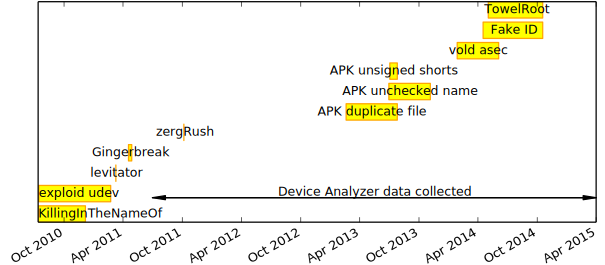
\includegraphics[width=\columnwidth]{figures/vulnerabilities_timeline}
 \caption{Timeline of vulnerabilities}
 \label{fig:vulnerabilities_timeline}
\end{figure}

The dates of discovery of vulnerabilities in the \avo\ is not uniform.
Figure~\ref{fig:vulnerabilities_timeline} shows the dates of discovery and, when later, the dates when a version of Android which fixed the vulnerability was shipped.
Some vulnerabilities (RageAgainstTheCage adb, levitator, zergRush abd TwerkMyMoto) were fixed in released versions of Android before they were discovered and so are shown as vertical lines while others were known for months before a version of Android which fixed them was shipped.
During the period in which \da\ data was collected the date when a version of Android with the fix was observed on a \da\ device is taken as the date that version was released, before that the release date as best as we can determine is used.
There is no canonical source of Android release dates, our best guesses and supporting references are available from \avo.

This data shows a large gap in the middle where we do not know of any discoveries of root equivalent vulnerabilities affecting all of Android.
The cause of this quiet period is unclear, perhaps from Figure~\ref{fig:proportioninsecure} the reason was that since most devices were exposed to known vulnerabilities there was no point in looking for new ones?
Or that manufacturers made it easier to install custom versions of Android, reducing the need for users to root their devices?
Or that manufacturer specific vulnerabilities (which we are ignoring) proved to be easier to find and so people looking for vulnerabilities adjusted their focus?

\section{Android Ecosystem}
There is a complex Android ecosystem which creates and distributes updates to Android which fix vulnerabilities.
It is also hard to quantify due to lack of public information on aspects of the ecosystem such as the number of manufacturers and updates.
We describe and quantify this ecosystem.

\subsection{Running a version of Android known to be vulnerable makes a device vulnerable}
We have not tried to exploit these vulnerabilities on the devices in order to test whether the devices are actually vulnerable.
Doing so would be difficult both ethically, as it would pose a high risk to user devices and mean that our code could easily be maliciously repurposed, and practically as getting all the exploits working reliably on all the devices they could be made to work reliably on requires extensive testing.
We are confident that most devices will be vulnerable if they are running a version of Android known to be vulnerable. \todo{WHY?}


\subsection{Android update process}

\label{sec:android_update_process}
\begin{figure}
 \centering
 \def\svgwidth{\columnwidth}
 \import{figures/}{update_ecosystem.pdf_tex}
 \caption{Flow of updates between participants in the Android ecosystem.
 Numbers on edges indicate updates shipped between \daStartDate\ and \daEndDate, numbers in brackets represent number of such entities in our data.
 Dotted arrows indicate flows where we do not know how many updates are being produced as we can't measure those flows directly as they are not public.}
 \label{fig:update_ecosystem}
\end{figure}
To understand how vulnerabilities in Android are fixed we must examine the Android update process which we model in Figure~\ref{fig:update_ecosystem}.
There are five entities or groups which contribute towards Android updates: the network operators, the device manufacturers, the hardware developers, Google and the upstream open source projects.
Android builds on various open source projects such as the Linux kernel, the OpenSSL and BouncyCastle cryptography libraries and so can include any compatible versions of those projects, including those which fix security vulnerabilities in them.
Android also incorporates various drivers for different bits of hardware.
The Android platform is then built on top of those with kernel and userspace components by Google.
The code for each update is kept secret\footnote{\url{https://source.android.com/source/code-lines.html}}\todolater{Can we quantify this keeping the code secret? Is it worth it?} until after the update has been published.
Manufacturers may receive advanced copies in order to prepare handsets.
Then the Manufacturers take the update and customise it before passing it on to the operator.
The Operator may then make further customisations and do further testing before shipping the update to the Device.
Sometimes Manufactures ship direct to the user, sometimes the Manufacturer and Google are the same entity (at least for the purpose of a particular phone, such as with Nexus phones).
Sometimes Manufacturers incorporate upstream open source project releases directly, and sometimes incorrectly -- for example including a broken daily build of sqlite in their release of Android
%An analysis by Vidas et al.~\cite{Vidas2011} of the Android 2.1 to 2.2 update found that it took 11 months from when Google released 2.2 for the last device which they were investigating to get the update.
\todolater{use statistics from samsung-updates.com -> how many binaries are there per device?}

The numbers of Devices (\daNumOSDevices), Operators (\daNumOperators) and Manufacturers (\daNumManufacturers) in Figure~\ref{fig:update_ecosystem} come from the \da\ data.
Manufacturer and Operator counts were obtained by normalising the results reported by Android to \da\ of the device manufacturer and active network operator.
This normalisation involves removing invalid values (such as `manufacturer' or `airplane mode is on'), collating across company name changes (e.g.\ `lge' to `lg'), normalising punctuation, removing extra strings sometimes added such as (`(2g)' or `communications') and mapping some incorrectly placed model names back to their manufacturer.
This normalisation is not perfect and so these are overestimates on the \da\ data but they are likely still underestimates as there will be some manufacturers and operators which are not included in the \da\ data.

The number of updates received by devices (\daNumFullVersions) is the number of different full version strings observed in \da.
The number of updates shipped by Google (\daNumSigOSVersions) is the number of Android versions reported in \da\ which affected more than \daSigVersionPerc\ of devices for more than \daSigVersionDays\ days. \todolater{this is the wrong number to be using}

We extracted data on the external projects used in Android and have included this and the scripts which generated it in \avo.
These scripts analysed the Android Open Source Project's source tree to examine the source code of each of the external projects to find the project version associated with each Android version tag on the repository.
There are \avoNumExternalProjects\ external open source projects in Android, contributing \avoTotalExternalLines\ lines of code.\footnote{Lines of code were measured using David A. Wheeler's \texttt{sloccount}.}
We analysed the top \avoNumBigExternalProjects\ by lines of code (contributing \avoNumBigExternalLinesOfCode\ lines, \avoBigExternalLinesOfCodePerc\ of the total) and were able to automatically extract the versions of those projects included in different versions of Android for \avoNumAnalysedExternalProjects\ (contributing \avoNumAnalysedExternalLinesOfCode\ lines, \avoAnalysedExternalLinesOfCodePerc\ of the total).
We found \avoBigExternalTotalVersions\ distinct versions, a median of \avoBigExternalMedianVersions\ and mean of \avoBigExternalMeanVersions\ versions per project.
This shows that Android rarely changes the version of external projects it includes.

To compute the latency between upstream releases and their inclusion in Android we scraped the release pages for those projects, to obtain the version numbers and release dates.
This allows us to compute the latency between an upstream project being released and it being included in Android, this is shown in Table~\ref{tab:update_ecosystem}.
This shows that the versions included in Android were about half a year old when that version of Android was released.
\begin{table}
\centering
\begin{tabular}{l|r|r}
Project	&	\# releases	&	latency \\ \hline
linux	&	\linuxNumVersions	&	\linuxMeanUpdateLatency \\
openssl	&	\opensslNumVersions	&	\opensslMeanUpdateLatency \\
bouncycastle	&	\bouncycastleNumVersions	&	\bouncycastleMeanUpdateLatency \\
\end{tabular}
\caption{Flow of updates from upstream projects into Android. Number of updates as in Figure~\ref{fig:update_ecosystem}, latency in days for all pairs of versions we have data on.\todolater{scrape the other 26 websites... is it worth it?}}
\label{tab:update_ecosystem}
\end{table}



\subsection{Monetisation of malware}
Android malware can make money in a variety of different ways~\cite{Felt2011}.
One of the key differences between smartphones and desktops is that it is easier to directly cash out on a smartphone as malware can send premium rate texts or make premium rate phone calls or send SMS and email spam.
It can also steal personal data which already has semantic information associated with it, this also makes it easier to sell and to perform ransomware attacks where malware deletes this information from the device and charges a ransom for its return.
It can steal credentials for external services or use in-app billing.
It can also do more conventional things such as use the devices for DDoS, SEO or click fraud attacks and altering the ads displayed to send the fees to the malware author.
While many of these things can be done by malware which just requests the relevant permissions, root exploits make this easier, particularly for ransomware and altering the ads displayed.

\subsection{Incentives and participants}
\label{sec:economics}
Google and other Android vendors care about the reputation of Android, particularly from a security standpoint as if users are afraid to use their devices for certain purposes (e.g.\ banking) then they will not be willing to pay as much for them and money cannot be made from those activities.
Manufacturers make money by selling the device, once sold they want to prevent the cost of return under warranty and so are adverse to the risk of breaking the device, but they do not need to do things to make the device better as it has already been sold.
However if they gain a reputation for abandoning devices that might decrease future sales.

Operators sell phones under contracts, typically at least a year long, they want the user to not request support due to the device breaking.
They might also gain advantage if the user is happy with the device after the end of the contract as they might then keep paying the same rate but there would no longer be a capital cost to pay off.
They care about phones not getting malware which causes support requests or uses the mobile network to perform malicious actions as they may have to reimburse the cost of premium SMS's if they were not authorised by the user.

Users want to buy phones which will serve their use cases and which are secure so that they do not experience negative consequences.


\section{Experiments}
\label{sec:results}
In this section we present the results of our analysis showing \daMeanInsecurityPerc\ of devices to have root equivalent vulnerabilities on average. Nexus devices are better than others, \emph{\daSecScoreBestmanufacturer} to be the best manufacturer and \emph{\daSecScoreBestoperator} to be the best network operator. \todo{ summarise our results}
%\todo{comparison of nexus update rates with iOS}
We conducted four experiments examining the behaviour of the Android ecosystem as a whole (\S\ref{sec:exp:android_ecosystem}), updates reaching particular devices (\S\ref{sec:exp:device_updates}), comparisons between different manufacturers and operators (\S\ref{sec:exp:security_score}) and model how long it will take for an update to be fixed once an update is released (\S\ref{sec:exp:predicting_distributions}).
\todo{In an experiment you test a hypothesis, it needs to be clear what the hypothesis is and what the conclusion of the test is}


\subsection{Experiment 1: behaviour of the Android ecosystem}\label{sec:exp:android_ecosystem}

\subsubsection{Method}
To investigate the behaviour of the Android ecosystem as a whole with respect to Android versions and vulnerabilities we used the OS version information from \da\ and the vulnerability data from \avo.
The \da\ data used here was collected between \daStartDate\ and \daEndDate.
The \avo\ data was collected between \avoStartDate\ and \avoEndDate\ and covers the period from \avoFirstDataDate\ to \avoLastDataDate.
We verify the validity of the \da\ data in \S\ref{sec:representative}.

\subsubsection{Results}
The proportion of devices in the \da\ data running different versions of Android each day is shown in Figure~\ref{fig:norm_os}.
It shows how old versions are gradually replaced by new ones, the long tail of devices which do not see updates to more recent versions and the fluctuation in the number of devices in the data.

\begin{figure}
 \centering
 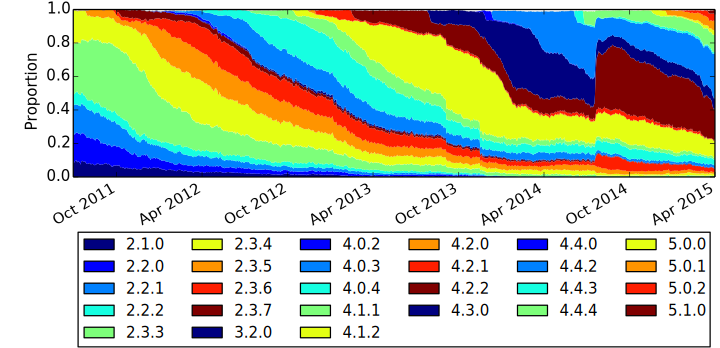
\includegraphics[width=\columnwidth]{figures/da_norm_os}
 \caption{Android versions in \da\ data over time}
 \label{fig:norm_os}
\end{figure}

Figure~\ref{fig:vulnerabilities} shows which vulnerabilities devices are exposed to.
For each vulnerability it shows the proportion of devices exposed to that vulnerability and how that changes over time.
In July 2011 at the beginning of the \da\ data the \emph{exploid}\footnote{\url{http://androidvulnerabilities.org/vulnerabilities/exploid_udev}} and \emph{levitator}\footnote{\url{http://androidvulnerabilities.org/vulnerabilities/levitator}} vulnerabilities both affect most Android devices, slowly these are fixed as updates roll out and devices are replaced until in January 2013 a much smaller proportion of devices are affected by known vulnerabilities.\todo{Quantify whether it is replacement of updates which causes the fixes}
However when in February 2013 the first APK signing vulnerability was found which affected all previous versions of Android and even in October 2013 most devices were still vulnerable. \todo{put percentages on these things to quantify them}
\begin{figure}%[!b]
\centering
\includegraphics[width=\columnwidth]{figures/vulnerabilities}
\caption{Proportion of devices exposed to each vulnerability with time (1.0 is 100\%)}
\label{fig:vulnerabilities}
\end{figure}

The variation of the proportion of devices affected by a vulnerability with time tells us how bad a particular vulnerability affected the Android platform.
Figure~\ref{fig:nvulnerabilities_heat} breaks this down by vulnerability to show how the proportion of devices affected by different vulnerabilities varies.
In 2013 three vulnerabilities were found in the way which Android verified the signatures on APKs.
These allowed the creation of malicious APKs which appear to be signed as system APKs -- which have root equivalent privileges.
Figure~\ref{fig:nvulnerabilities_heat} shows how the the \emph{APK signing vulnerabilities} affected all devices and took months to get fixed for any device.
However what is perhaps more worrying is the long tail on the \emph{Gingerbreak}\footnote{\url{http://androidvulnerabilities.org/vulnerabilities/Gingerbreak}}, \emph{levitator} and \emph{exploid} vulnerabilities which are more dangerous root vulnerabilities (not requiring new APK installation) and which still affect a significant proportion of devices years later.
\todo{break things down by attack vector?}

\begin{figure}
 \includegraphics[width=\columnwidth]{figures/nvulnerabilities_heat.pdf}
 \caption{Proportion of devices affected by different vulnerabilities}
 \label{fig:nvulnerabilities_heat}
\end{figure}


\subsection{Experiment 2: Updates to particular devices}\label{sec:exp:device_updates}
Those graphs summarise data across all the devices, however one of the advantages of the \da\ data is that it allows us to look at what happens to individual devices over time.
\subsubsection{Method}
\todo{write a method}
\subsubsection{Results}
Figure~\ref{fig:device_data} shows how the number of vulnerabilities affecting the \daNumDeviceDataDevices\ devices which have contributed the most days of data to \da\ changes over time.
The trend that we saw in Figure~\ref{fig:proportioninsecure} of security improving and then getting worse is also shown here.
It shows how some devices had vulnerabilities, which were fixed, and then further vulnerabilities were discovered, and for these devices, mostly not fixed.
\begin{figure}
 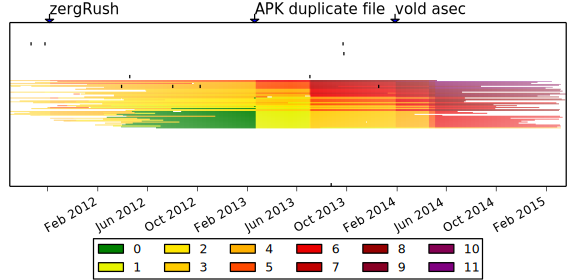
\includegraphics[width=\columnwidth]{figures/device-data-all-security}
 \caption{Number of vulnerabilities affecting the top \daNumDeviceDataDevices\ devices by days of contribution in the \da\ data}
 \label{fig:device_data}
\end{figure}

\subsubsection{Update frequency}
\todo{ find out what the frequency of updates is}
\begin{figure}
 \includegraphics[width=\columnwidth]{figures/from_to_updates.pdf}
 \caption{Updates between different Android versions in the \da\ data}
 \label{fig:from_to_updates}
\end{figure}
\begin{figure}
 \includegraphics[width=\columnwidth]{figures/w_security_updates.pdf}
 \caption{Number of updates each week which fixed or may have fixed security vulnerabilities}
 \label{fig:weekly_security_updates}
\end{figure}
Figure~\ref{fig:from_to_updates} shows how devices upgrade between different versions of Android.
\da\ observes upgrade events and the figure shows which versions a device is upgrading from and to.
Mostly the dark cells are above the diagonal and are upgrades (\daNumUpdatesUpgrades).
While many upgrades are from one version to the next version there are also a fair number which skip a few versions.
Surprisingly there are also a small number of downgrade events (\daNumUpdatesDowngrades, \daPercUpdatesDowngrades) when older versions of Android are installed on to devices.
Possible reasons why users are downgrading are to free up space on their device, to make it easier to root or because a new version introduced bugs.

The number of devices getting security updates each week, is shown in Figure~\ref{fig:weekly_security_updates}, blue shows updates which changed the Android version number from a version with known vulnerabilities to one which had fewer known vulnerabilities.
Red indicates updates which changed the build number but not the version number and so might contain a backported fix for a vulnerability.
\todo{ summary stats, what does this mean}


\subsection{Scoring for security}
\label{sec:security_scoring}

Computing how good a particular manufacturer or device model is from a security standpoint is difficult as it depends on a number of factors which are hard to observe, particularly on a large scale.
Ideally we would consider both prevelance of potential problems which were not exploited and actual security failures.
However in the absence of such data we propose a scheme for assigning a device a score out of ten based on data which can be observed, and which hopefully correlates with the actual security of the devices.

This score is computed from several components:
\begin{description}
  \item[$i$] The proportion of the time were devices exposed to known vulnerabilities. This is equivalent to Acer and Jackson's proposal~\cite{Acer2010} to measure the security based on the proportion of users with at least one unpatched critical vulnerability and is also $1 -$ the Vulnerability Free Days score~\cite{Wright2014}.
  \item[$u$] The proportion of devices run the latest version of Android shipped to any device produced by that manufacturer. This is a measure of internal updatedness, a low score would mean many devices are being left behind.
  \item[$m$] The mean number of outstanding vulnerabilities affecting devices not fixed on any device shipped by the manufacturer. This is related to the Median Active Vulnerabilities measure~\cite{Wright2014} but is the mean rather than the median.
%TODO should we compute the median instead?
\end{description}
\begin{equation}
\mathrm{score} = (1 - i)\times 4 + u \times 3 + \frac{2}{1+e^m} \times 3
\end{equation}

The scores accross the whole of android are that \daMeanInsecurityPerc\ of devices are exposed to known root exploits.
There are on average \daMeanOutstandingVulnerabilities\ outstanding vulnerabilities not fixed on any device.
Only on average \daUpdatednessPerc\ of devices run the most recent version of Android.
This gives a security score of \daSecurityScore/10.
\daTabSecScoressummary
However there are a wide variety of scores depending on the source of the device.
There have been many reports that Google's Nexus devices are better at getting updates than other Android devices because Google makes the original updates and ships them to its devices.
Table~\ref{tab:sec_summary} shows that this is the case with Nexus devices getting much better scores than non-Nexus devices.
\daTabSecScoresmanufacturer
Different manufacturers have very different scores, Table~\ref{tab:sec_manufacturer} shows the scores for the \daNumSigManufacturers\ manufacturers with a significant presence in our data.
Manufacturers are considered significant if we have data from at least \daSigNumDevices\ devices and at least \daSigNumDays\ days of contributions.
\daTabSecScoresmodel
Even within manufacturers different models can have very different update behaviours and hence security.
Table~\ref{tab:sec_model} shows the results for the \daNumSigModels\ device models which have a significant presence by the same metric.


% We don't need this for this paper
%\subsection{Comparison with iOS}
%\todo{Get data from Richard so that we can do this comparison}


\subsection{Experiment 4: Predicting future version distributions}\label{sec:exp:predicting_distributions}
\subsubsection{Method}
Examining the way that the OS version distribution changes over time in Figure~\ref{fig:norm_os} we see some regularity to the behaviour.
To show this behaviour more clearly we normalised the data to the number of days since the version was released and smoothed it by forcing it to be monotonically decreasing.\footnote{While sometimes an older version becomes more popular after a later version has been released causing the values to actually increase, mostly this was just noise or changes in the distribution of devices (e.g.\ the sudden arrival of 1000 devices from Bangladesh due to a study being conducted there) and this assumption makes the graph clearer.}
Then we can plot Figure~\ref{fig:frvh_os_versions} which shows the proportion of of devices in \da\ not upgraded to each Android version or a later Android version (i.e. for 2.1.0 it includes 2.1.1, 2.2.0 and indeed all devices as they all run later versions of Android).
The mean and standard deviation of the same data are shown in Figure~\ref{fig:frms_os_versions}.

\begin{figure}
 \includegraphics[width=\columnwidth]{figures/frvh_os_versions}
 \caption{Proportion of devices not updated to particular versions of Android or any later version\todo{make line of best fit thicker, I think the drops to 0 at the end of each version are erroneous}}
 \label{fig:frvh_os_versions}
\end{figure}
\begin{figure}
 \includegraphics[width=\columnwidth]{figures/frms_os_versions}
 \caption{Proportion of devices not updated to particular versions of Android or any later version}
 \label{fig:frms_os_versions}
\end{figure}

The data appears to have an exponential decay as it tends to 1 but with a slow start as few devices are upgraded initially.
We approximate this with a $e^{-x}$ for the main behaviour and a which is offset to start later when uptake takes off.
The equation is then:
\begin{equation}
y =
 \begin{cases}
  1.0 & \text{if }x<\mathrm{undeployed}\\
  e^{-\mathrm{decay}(x-\mathrm{undeployed})} & \text{otherwise}
 \end{cases}
\end{equation}

\subsubsection{Results}
Fitting that curve to the data using \texttt{scipy.optimize}, we get a RMSE of \daOSCurveFitRMSE\ and parameters $\mathrm{undeployed} = \daOSCurveFitParamFirst ~\si{days}$, $\mathrm{decay} = \daOSCurveFitParamSecond ~\si{days^{-1}}$ for OS versions and RMSE of \daAPICurveFitRMSE\, $\mathrm{undeployed} = \daAPICurveFitParamFirst ~\si{days}$, $\mathrm{decay} = \daAPICurveFitParamSecond ~\si{days^{-1}}$ for API versions.
From this the number of days from release of a new version of Android until 50\% of devices are running that version or higher is \daOSCurveHalfDeployed\ and full deployment to \daFullDeployedAt\ of devices takes \daOSCurveFullDeployed\ days.
For API versions this is \daAPICurveHalfDeployed\ and \daAPICurveFullDeployed\ respectively.

Hence if a security vulnerability is fixed through the release of a particular Android version it will be \daOSCurveFullDeployed\ days after until the fix is fully deployed.

The equation we chose for the model has a root mean squared error (RMSE) of \daOSCurveFitRMSE\ for OS versions, which is a comparably good fit to a standard polynomial fit (3 degree polynomial fit gave a RMSE of \daOSCurvePolyRMSE) or a spline fit (RMSE of \daOSCurveSplineRMSE) but gives a meaningful model of behaviour rather than a generic curve.

\todo{Evaluate our model trained on the DA data against the ground truth Google Play data}

\todo{Our handling of errors here is not quite good enough as the uncertainty from our y value interacts badly with the logarithm function when computing the inverse and we compute the log of ~0 which means our error ends up much bigger than our value - but that is an upper bound, not a +- bound.}

We hope that a consequence of this paper will be a change in behaviour of the Android ecosystem which invalidates this model by speeding up the deployment of new OS versions.

\section{Threats to validity}
\subsection{The \da\ data gives a conservative estimate of the Android version distribution}
\label{sec:representative}
\begin{figure}
 \centering
 \begin{subfigure}[b]{\columnwidth}
 \includegraphics[width=\columnwidth]{figures/googleplayapi}
 \caption{Google Play data on proportion of devices running different Android API versions}
 \label{fig:play_api}
\end{subfigure}
\begin{subfigure}[b]{\columnwidth}
 \includegraphics[width=\columnwidth]{figures/norm_api_gpcomp}
 \caption{\da\ data on proportion of devices running different Android API versions}
 \label{fig:da_api}
\end{subfigure}
\caption{Monthly Android API version data}
\end{figure}
\begin{figure}
 \centering
 \includegraphics[width=\columnwidth]{figures/api_gpcomp_rdiff}
 \caption{Difference between \da\ and Google Play data on the proportion of devices running different Android API versions}
 \label{fig:da_gp_comp_diff}
\end{figure}
The data from \da\ (DA) we used to investigate the proportion of devices exposed to different vulnerabilities is the OS version.
Unfortunately there is no authoritative source of OS version information and so we cannot check directly whether our data is representative.
However Google has published API version information every month since December 2009 and we have collated this information.\footnote{\url{https://www.cl.cam.ac.uk/~drt24/android/versiondistribution/}}
While API versions are too coarse grained to use for security update detection they are closely related to OS versions and so if the \da\ data on API versions is similar to the Google Data on API versions then the \da\ data on OS versions should be representative.
Figure~\ref{fig:play_api} shows the data from Google and Figure~\ref{fig:da_api} shows the data from \da\ and they appear similar.
Figure~\ref{fig:da_gp_comp_diff} shows the difference between Figures~\ref{fig:play_api} and \ref{fig:da_api}, normalising for days since the API version was released.
It shows that the \da\ data systematically overestimates the prevalence of new API versions and underestimates the prevalence of old API versions.
This means that the OS version information from \da\ is likely to be overestimating the prevalence of new OS versions and hence our results are a conservative estimate of the security of Android.
\todo{we want a statistical metric to claim this strongly with.}
This allows us to have confidence in the OS version information.


\subsection{Changes in the \da\ sample}
\todo{Bangladesh etc.}

\subsection{Uncertainty propagation}

\section{Discussion}
There are continuing efforts to reduce the impact of root equivalent vulnerabilities, both in Android and more widely.
SEAndroid~\cite{Smalley2013} which is included in Android from version 4.1~\cite{jelly-bean-release} claimed to prevent some root vulnerabilities and to reduce the impact of others.
Capability based enforcement systems such as Capsicum~\cite{Watson2010} substantially reduce the capabilities that an exploit has to try and gain increased privilege with.
When Capsicum is included in Linux~\cite{TODO} and hence in Android, it could be used to place fine grained restrictions on system daemons, preventing vulnerabilities becoming root equivalent vulnerabilities.


\subsection{Open questions}
\begin{itemize}
 \item Why was there a gap in vulnerability discovery in Android in 2012?
 \item Why do so many devices have ADB enabled?
 \item How much of updating is new handsets and how much is updates being deployed?\todo{we should answer this question in this paper}
 \item Why do users downgrade their phones?
\end{itemize}


\section{Related work}
\label{sec:related}
We found that since 2011 \daMeanInsecurityPerc\ of devices on average were exposed to known root equivalent vulnerabilities.
In 2011 Felt et al.\ \cite{Felt2011} studied 6 Android handsets and found that they were exposed to root vulnerabilities at least 74\% of the time.
This might indicate that over the last 3 years the security of Android has not improved, but these data are not directly comparable as their study was on 6 handsets considering the best possible update distribution while ours is on a large sample of devices with the real update distribution.
They also found that 4 of the 46 malware samples (8\%) they analysed contained root exploits, much lower than rates found in later larger studies which found rates of 36.7\%~\cite{Zhou2012b} and 40\%~\cite{Zhou2012a}.
Perhaps the malware authors heard about the results in Felt et al.'s paper?
Our results show root exploits are still a severe threat.

Finding vulnerabilities is frequently a time consuming manual process but, Brumley et al.~\cite{Brumley2008} showed that it is possible to automatically generate exploits from binary patches.
In a similar way some of the vulnerabilities\todolater{which?} which have been exploited were publicly found by examining the commit made to the Android which fixed the vulnerability.
This effect has been observed before~\cite{Barth2011} in the Firefox source code repositories, Google does not release the source code until after the release of the update reducing this effect to the delay between an update being released and it reaching the last end user device.
There have been other attempts to automatically find vulnerabilities.
The Woodpecker tool~\cite{Grace2012} automatically finds permission leaks in stock Android phone images.
The update process itself can allow Android apps to gain privilege through `Pileup' vulnerabilities~\cite{Xing2014} by registering for new permissions before the update which creates that permission is installed.

The security protections used in iOS such as only allowing signed code to run, jails and reviewing of apps has resulted in a lower level of malware affecting iOS~\cite{TODO} but can still be bypassed~\cite{Wang2013a}. \todo{look at iOS protections again and tighten this up}

Various attempts have been made to detect malware.
RiskRanker~\cite{Grace2012a} classified 3,281/118,318 (2.8\%) apps as risky of which 718 (22\%) were malware and 322 (10\%) were previously unknown malware, an infection rate of 0.6\% across multiple markets.
It uses signatures of exploits, static analysis of calls to high risk operations, detection of encrypted native code execution and dynamic Dalvik code loading to detect risky apps.
DroidRanger~\cite{Zhou2012a} found 148/182,823 (0.08\%) apps to be malicious across multiple markets of which 29 were previously unknown.
It used permission-based behavioural fingerprinting -- looking at the permissions of known malware and heuristic-based filtering -- dynamic loading of both Dalvik and native code.
AnDarwin~\cite{Crussell2013} detects similar apps, it found 169/265,359 (0.06\%) malicious apps based on the difference in permissions between the malicious app and the app which had been cloned.
It used clustering based on semantic vectors derived from the program dependence graphs to detect similar apps.
The Malware Genome project~\cite{Zhou2012b} collected 1,260 malware samples from 2010--2011.
They found that the best case for anti-malware detection on this data was 79.6\%.
However DroidChameleon~\cite{Rastogi2013} found that antivirus products could not detect malware if it was simply automatically permuted.
All these app analysis projects have been hampered by the difficulty of obtaining full datasets of Android apps as Google does not make these available (and researchers who automatically download them, violate Google's Terms of Service).
PlayDrone~\cite{Viennot2014} was a particularly effective project which circumvented Google's protective measures and downloaded over 1,100,000 apps from Google Play, allowing an in depth analysis.

Examining security updates has been a key way of assessing security for many years.
Many software update systems have been found not to authenticate the connection to the update server and/or do not authenticate the downloaded binaries~\cite{Bellissimo2006}.
Even package management systems designed to provide secure updates have been found to have vulnerabilities~\cite{Cappos2008}.
Fortunately Android does authenticate the update binaries (though the APK vulnerabilities circumvented this) and Google Play downloads them over a secure connection~\cite{Viennot2014}. \todolater{double check that}

The updatedness rate for Android of \daUpdatednessPerc\ compares unfavourable with the more than 90\% rate for Windows XP SP2 computers contacting the Microsoft update servers~\cite{Gkantsidis2006} though that is within one OS version and only for those computers which did connect to the servers -- but that is the default.
However 27\% of Windows computers were still running Windows XP in July 2014\footnote{\url{https://archive.today/PLGxn}\todolater{Get updated figures before publication}} -- four months after it went out of security support.

User-Agent strings have been used to investigate how web browser versions change with updates~\cite{Frei2008} and found that at most 80\% of Firefox users were running the most recent version.
The same analysis was used to show that Chrome's use of silent updates seems to increase uptake of upgrades~\cite{Duebendorfer2010} with 97\% of users running the latest version within 3 weeks of release.
Android's update process is manual, the user is notified but must action the upgrade which will then download the update and install it, the phone is rendered inoperable during the update process which is inconvenient for users and the phone must have sufficient charge so that it will not run out during the update process.
Partly this is the result of the fact that an operating system update is being installed and so a reboot is required, but Chrome installs the new version side by side with the old one and switches the next time it is restarted.
The same technique would be more difficult on phones with limited storage space (as for many cheap Android phones which have barely enough space to install just the update) but is a plausible improvement for more high-end devices.
Google is deploying the same silent update technique through Google Play Services~\cite{TODO} which automatically installs updates for core Google components of Android, this also bypasses the manufacturer and operator.



\section{Conclusion}
\label{sec:conclusion}
\todo{Conclude}


\section*{Acknowledgements}
Thanks to David Robertson for helpful advice on statistical analysis.
Thanks to Laurent Simon, Thomas Coudray, Adrian Taylor, Justin Case and Khilan Gudka for reporting vulnerabilities in Android.

\printbibliography


\end{document}
